% questions.tex —— 1977 年·湖北卷 · 题目内容片段（无答案）
% 由 tools/generate_projects.py 依来源总账自 1977/1977_数学真题_湖北_试题.md 生成，勿手改（改源 MD 后重跑）


\gkpart{数学试题解（湖北卷）}

\begin{gktip}
\textbf{来源说明}：本题面依据固定源 PDF《湖北1977年高考数学试题解》第 1—5 页（书页 92—96）逐题转录。固定源是题面与解答连续出现的扫描材料，每题题面之后紧接「解」，不是无答案试卷；配套答案与解析对照源解答独立复算，\textbf{非官方标准答案}。正式题为第一—五大题，末尾「参考题」三题原卷注明不计入考分，只供录取后参考。原卷未出现文理分科说明。原卷大题以汉字「一、二、三、四、五」编号，本库题库规范要求阿拉伯数字题号，故对应重排为第 1—5 题，第一题下的 8 个小题保持（1）—（8）编号不变。
\end{gktip}

\par\medskip

\begin{question}
\gkti{1}\textbf{（每小题 5 分，共 40 分）} 计算：

（1） $\sqrt{(-3)^2}$；$\sqrt[3]{(-27)^3}$．

（2） $\log_2 2+\log_5 1-\log_{\frac13}\frac{1}{27}$．

（3） $\left(\sqrt{\dfrac23}\right)^3\cdot\sqrt[3]{\left(\dfrac32\right)^2}\cdot\left(\dfrac23\right)^{-\frac56}$．

（4） 解方程：$x-\sqrt{8-x^2}=0$．

（5） 当 $m\leqslant 1$ 时，计算 $\sqrt{(m-1)^2}$．

（6） 求函数 $y=\dfrac{\sqrt{2-x}}{x+4}$ 的定义域．

（7） 分解因式：$x^4+x^2y^2+y^4$．

（8） 证明：$\operatorname{tg}22^\circ30'=\sqrt2-1$（不查表）．

\Needspace{0.4\textheight}
\end{question}
\begin{question}
\gkti{2}\textbf{（10 分）} 围一矩形场地，一边利用房屋的墙，其他三边用 $L$ 米的篱笆围成，问怎样围才能使面积最大？最大面积是多少？

\begin{gktip}
原源 PDF 第 3 页附有矩形场地与房屋墙的示意图；LaTeX 版按源图重绘。
\end{gktip}
\nopagebreak[4]
\begin{center}% 1977 年湖北卷第二题：矩形场地一边靠房屋的墙（斜线段示墙），平行于墙的一边长标 x（按源卷第 3 页布局）
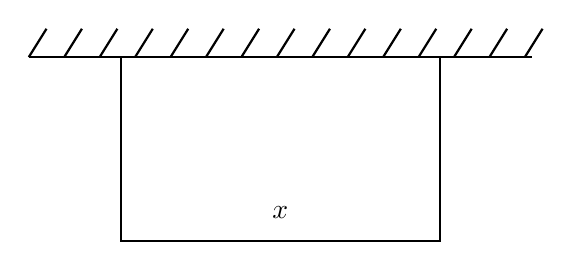
\begin{tikzpicture}[scale=0.9]
  \draw[thick] (0,0) rectangle (4.5,2.6);
  \draw[thick] (-1.3,2.6)--(5.8,2.6);
  \foreach \i in {0,...,14}
    \draw[thick] ({-1.3+0.5*\i},2.6) -- ({-1.05+0.5*\i},3.0);
  \node at (2.25,0.4) {$x$};
\end{tikzpicture}
\end{center}
\nopagebreak[4]
\end{question}
\begin{question}
\gkti{3}\textbf{（10 分）} 已知直线 $L_1$ 方程为 $x+y-1=0$ 和点 $A(-3,0)$．

（1） 求与直线 $L_1$ 垂直且通过 $A$ 的直线方程；

（2） 求点 $A$ 到直线 $L_1$ 的距离．

\end{question}
\begin{question}
\gkti{4}\textbf{（20 分）} 解方程组：

\nopagebreak[4]
\[
\begin{cases}
\operatorname{Log}_2 x-\operatorname{Log}_4 y=0,\\
y^2-13x^2+36=0.
\end{cases}
\]

\end{question}
\begin{question}
\gkti{5}\textbf{（20 分）} 作函数 $y=\sqrt3\cos 2x+\sin 2x$ 的图象（要求写出作图步骤，并画出草图）．

\begin{gktip}
\textbf{参考题}（不计入考分，只供录取后参考）
\end{gktip}

\Needspace{5\baselineskip}
\textbf{参考题 1．} 求下列函数的导数：

\nopagebreak[4]
\[
y=\sin x;\qquad y=\mathrm e^{3x};\qquad y=\operatorname{Ln}x;\qquad f(t)=A\sin(\omega t+\varphi).
\]

\textbf{参考题 2．} 设函数 $f(x)=x^3-12x+10$．

（1）求 $f(x)$ 的极值点；

（2）求 $f(1)$，$f(2)$，$f(-3)$．

\Needspace{5\baselineskip}
\textbf{参考题 3．} 解方程：

\nopagebreak[4]
\[
\begin{cases}
y''+3y'-4y=0,\\
y\big|_{x=0}=0,\\
y'\big|_{x=0}=-10.
\end{cases}
\]

\end{question}